\documentclass{article}
\usepackage{tikz, comment}
\usepackage{pifont}
\usepackage{fontspec}
\usetikzlibrary{arrows, decorations.markings, decorations.pathreplacing}
\begin{comment}
:Title: Not defined yet
:Tags: eccentricity of a conic section;focus of a parabola;focal radius ;perimeter;directrix of a parabola
:Prob: 0.6035;0.5731;0.561;0.5583;0.5567
:Author: Prof.Hu Ji-shan, HKUST
:Slug: No name yet

Description Here.........
\end{comment}
\begin{document}\centering

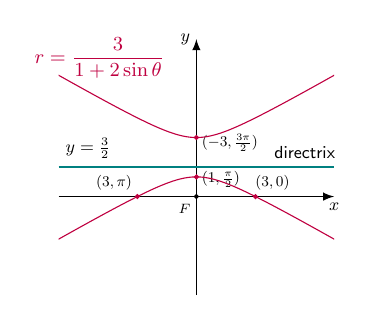
\begin{tikzpicture}[>=latex,xscale=.5/2, yscale=.5/2][font=\sf\small]

%\draw[xstep=1cm,ystep=1cm,color=gray!80] (0, -1) grid (8, 8);

\draw[->] (-7, 0) -- (7, 0)node[below, scale=0.7] {$x$};
\draw[->] (0, -5) -- (0, 8)node[left, scale=0.7] {$y$};

\draw[teal, samples=100, smooth, domain=-7:7, variable=\x]
plot ({\x}, {3/2});

\node[above, xshift=0, yshift=0, scale=0.7] at (-5.5,{8/5}) {$y=\frac{3}{2}$};
\node[above, xshift=0, yshift=0, scale=0.7] at (5.5,{8/5}) {$\hbox{directrix}$};

\node[purple, xshift=-35, yshift=50, scale=0.8] at (0,0) {$\displaystyle r = \frac{3}{1+2\sin \theta}$};

\draw[fill, xscale= 2, yscale= 2] ({0/1}, {0/1}) circle(0.05);

\draw[purple, fill, xscale= 2, yscale= 2] ({3/2}, {0/2}) circle(0.05)node[black, right, xshift=-2, yshift=5, scale=0.6] {$(3,0)$};

\draw[purple, fill, xscale= 2, yscale= 2] ({-3/2}, {0/2}) circle(0.05)node[black, left, xshift=0, yshift=5, scale=0.6] {$(3,\pi)$};

\draw[purple, fill, xscale= 2, yscale= 2] ({0/2}, {(3)/2}) circle(0.05)node[black, right, xshift=0, yshift=-2, scale=0.6] {$(-3,\frac{3\pi}{2})$};

\draw[purple, fill, xscale= 2, yscale= 2] ({0/2}, {1/2}) circle(0.05)node[black, right, xshift=0, yshift=-1, scale=0.6] {$(1,\frac{\pi}{2})$};

\foreach \x in {}
\draw (\x,2pt*2) -- (\x,-2pt*2)
node[anchor=north] {}%{\tiny$\x$}
;
\foreach \x in {}
\draw (\x,2pt*2) -- (\x,-2pt*2)
node[anchor=south] {\tiny$\x$}
;
\foreach \y in {}
\draw (-2pt*2,\y) -- (2pt*2,\y)
node[anchor=east] {}%{\tiny $\y$}
;

\node[scale=0.7] at ({-0.2*1.5*2}, {-0.2*1.5*2}) {\scriptsize$F$};

\clip[] (-7, -4.5) rectangle (7, 8);
\draw[purple, samples=100, smooth, domain=3*pi/2-1:3*pi/2+1, variable=\t]
plot ({3/(1+2*sin(\t r))*cos(\t r)}, {3/(1+2*sin(\t r))*sin(\t r)});

\draw[purple, samples=100, smooth, domain=pi/2-2:pi/2+2, variable=\t]
plot ({3/(1+2*sin(\t r))*cos(\t r)}, {3/(1+2*sin(\t r))*sin(\t r)});

\end{tikzpicture}
\end{document}